\documentclass[12pt,a4paper]{article}

% =========================================================
% 1. CẤU HÌNH TÀI LIỆU CHUNG
% =========================================================
\usepackage[utf8]{vietnam}
\usepackage{amsmath,amssymb}
\usepackage{geometry}
\usepackage{graphicx}
\usepackage{booktabs}
\usepackage{array}
\usepackage{xcolor}
\usepackage{float}
\usepackage{setspace}
\usepackage{hyperref}

% Cấu hình tài liệu tham khảo với BibLaTeX (Biber)
\usepackage[backend=biber,style=numeric]{biblatex}
\addbibresource{references.bib}

\geometry{
    left=2.5cm,
    right=2.5cm,
    top=2.5cm,
    bottom=2.5cm
}

\hypersetup{
    colorlinks=true,
    linkcolor=black,
    citecolor=blue,
    urlcolor=blue,
    pdftitle={Computer Project Report},
    pdfauthor={Group 3}
}

\onehalfspacing
\setlength{\parindent}{1cm}
\setlength{\parskip}{0.3em}
\setlength{\emergencystretch}{2em}

\renewcommand{\contentsname}{Mục lục}

% Các lệnh tự tạo (giữ nguyên từ file cũ của bạn)
\newcommand{\canbosung}[1]{%
    \textcolor{blue}{[Cần bổ sung: #1]}%
}

\newcommand{\chenhinh}[3]{%
    \begin{figure}[H]
        \centering
        \IfFileExists{#1}{%
            \includegraphics[width=0.85\textwidth]{#1}
        }{%
            \fbox{%
                \parbox[c][5cm][c]{0.82\textwidth}{%
                    \centering
                    \textbf{Vị trí chèn hình}\\[0.5em]
                    #2\\[0.5em]
                    Tên tệp: \texttt{\detokenize{#1}}
                }%
            }%
        }
        \caption{#2}
        \label{#3}
    \end{figure}
}

% =========================================================
% BẮT ĐẦU TÀI LIỆU
% =========================================================
\begin{document}

% =========================================================
% 2. TRANG BÌA
% =========================================================
\begin{titlepage}
    \centering

    \vspace*{1.5cm}

    {\Large\bfseries MAI391\par}

    \vspace{1.5cm}

    {\Huge\bfseries Computer Project Report\par}

    \vspace{1cm}

    {\Large
    Hồi quy tuyến tính đơn biến và Gradient Descent
    trên dữ liệu hiệu năng mạng
    \par}

    \vspace{1.5cm}

    {\large
    \textbf{Giảng viên:} Nguyễn Hoàng Tường Vy
    \par}

    \vspace{0.8cm}

    {\Large\bfseries Group 3\par}

    \vspace{0.5cm}

    \begin{tabular}{ll}
        \toprule
        \textbf{Họ và tên} & \textbf{Mã số sinh viên} \\
        \midrule
        Phan Lê Thanh Hùng & QE210207 \\
        Đinh Tấn Huy      & QE200063 \\
        Võ Quốc Tuấn      & QE200052 \\
        Phan Thành Đạt    & \canbosung{MSSV} \\
        \bottomrule
    \end{tabular}

    \vfill

    {\large \today\par}
\end{titlepage}

% =========================================================
% 3. MỤC LỤC
% =========================================================
\pagenumbering{roman}
\tableofcontents
\clearpage

\pagenumbering{arabic}

% =========================================================
% 4. GỌI NỘI DUNG 10 BÀI TỪ THƯ MỤC CHAPTERS
% (Mỗi thành viên chỉ sửa file tương ứng của mình)
% =========================================================
% =========================================================
% BÀI 1: GIỚI THIỆU BÀI TOÁN VÀ BỘ DỮ LIỆU
% =========================================================
\section{Giới thiệu bài toán và Bộ dữ liệu}

\subsection{Đặt vấn đề}
Nhằm đáp ứng yêu cầu số 1 của đồ án môn học: \textit{"Thu thập một bộ dữ liệu thứ cấp phù hợp (real-world secondary dataset) về một chủ đề liên quan đến công nghệ, chứa tối thiểu 500 quan sát"}, nhóm đã lựa chọn bộ dữ liệu giám sát hiệu năng mạng từ thực tế (Network Telemetry). 

Chất lượng kết nối mạng có thể biến động theo thời gian do lưu lượng truy cập, tình trạng đường truyền và các yếu tố hạ tầng. Những biến động này ảnh hưởng trực tiếp đến độ trễ (Latency), mức độ ổn định và trải nghiệm của người dùng. 

Mục tiêu của bài toán là dự đoán **độ trễ trung bình khi gửi và nhận gói tin tới máy chủ đích** (Round Trip Time - RTT) dựa trên các đặc trưng về mạng và thời gian. Trong phạm vi bài báo cáo này, nhóm tập trung xây dựng mô hình hồi quy tuyến tính đơn biến, sử dụng duy nhất một đặc trưng đầu vào để dự đoán độ trễ.

\subsection{Định nghĩa Input và Output}

Bài toán được thiết lập với một biến độc lập (Input) và một biến phụ thuộc (Output) như sau:

\begin{table}[H]
    \centering
    \caption{Định nghĩa các biến trong mô hình}
    \begin{tabular}{llp{0.5\textwidth}}
        \toprule
        \textbf{Loại biến} & \textbf{Tên cột (Feature)} & \textbf{Ý nghĩa} \\
        \midrule
        \textbf{INPUT (X)} & \texttt{gateway\_rtt\_avg\_ms} & Độ trễ trung bình tới Gateway (mili giây - ms) \\
        \addlinespace
        \textbf{OUTPUT (Y)} & \texttt{rtt\_avg\_ms} & Độ trễ trung bình khi gửi và nhận gói tin tới máy chủ đích (ms) \\
        \bottomrule
    \end{tabular}
\end{table}

\textbf{Lý do lựa chọn:} Cả hai đại lượng cùng phản ánh độ trễ mạng và có tương quan dương dự kiến. Độ trễ đến Gateway thường ổn định và dễ đo liên tục; nếu tồn tại quan hệ tuyến tính đủ mạnh, có thể dùng đại lượng dễ đo này để ước lượng độ trễ đến đích mà không phải gửi gói tin đến máy chủ từ xa trong mọi chu kỳ giám sát.

\subsection{Thu thập và tải dữ liệu}

Dữ liệu được thu thập từ bộ dữ liệu thứ cấp (định dạng CSV) lưu trữ trên Google Drive. Tệp dữ liệu chứa hơn \(54\,000\) quan sát (dòng), hoàn toàn thỏa mãn điều kiện tối thiểu \(500\) quan sát của đề bài. 

Quá trình tải và trích xuất dữ liệu được tự động hóa bằng ngôn ngữ Python (sử dụng thư viện \texttt{gdown} và \texttt{pandas}). Đoạn mã cốt lõi thực hiện tải dữ liệu và khai báo biến được minh họa như sau:

\begin{verbatim}
import gdown
import pandas as pd

# Tải file từ Google Drive
file_id = '1RgrGtIgDJQiuYjxZ3WSxESXdaZztoj9T'
download_path = 'dataset.csv'
gdown.download(id=file_id, output=download_path, quiet=False)

# Đọc dữ liệu
df = pd.read_csv(download_path)
print(f"Kích thước dữ liệu: {df.shape[0]} dòng, {df.shape[1]} cột.")

# Khai báo biến
X_feature = ['gateway_rtt_avg_ms']
target_y = 'rtt_avg_ms'
\end{verbatim}

Sau khi tải thành công, nhóm tiến hành kiểm tra sự tồn tại của các cột \texttt{gateway\_rtt\_avg\_ms} và \texttt{rtt\_avg\_ms} để đảm bảo dữ liệu sẵn sàng cho các bước tiền xử lý và phân tích khám phá (EDA) tiếp theo. % Giới thiệu bài toán & Bộ dữ liệu

% =========================================================
% BÀI 2: Thu thập và tải dữ liệu
% =========================================================

\section{Thu thập và tải dữ liệu}

Dữ liệu được thu thập từ bộ dữ liệu thứ cấp (định dạng CSV) lưu trữ trên Google Drive. Tệp dữ liệu chứa hơn \(54\,000\) quan sát (dòng), hoàn toàn thỏa mãn điều kiện tối thiểu \(500\) quan sát của đề bài. 

Quá trình tải và trích xuất dữ liệu được tự động hóa bằng ngôn ngữ Python (sử dụng thư viện \texttt{gdown} và \texttt{pandas}). Đoạn mã cốt lõi thực hiện tải dữ liệu và khai báo biến được minh họa như sau:

\begin{verbatim}
import gdown
import pandas as pd

# Tải file từ Google Drive
file_id = '1RgrGtIgDJQiuYjxZ3WSxESXdaZztoj9T'
download_path = 'dataset.csv'
gdown.download(id=file_id, output=download_path, quiet=False)

# Đọc dữ liệu
df = pd.read_csv(download_path)
print(f"Kích thước dữ liệu: {df.shape[0]} dòng, {df.shape[1]} cột.")

# Khai báo biến
X_feature = ['gateway_rtt_avg_ms']
target_y = 'rtt_avg_ms'
\end{verbatim}

Sau khi tải thành công, nhóm tiến hành kiểm tra sự tồn tại của các cột \texttt{gateway\_rtt\_avg\_ms} và \texttt{rtt\_avg\_ms} để đảm bảo dữ liệu sẵn sàng cho các bước tiền xử lý và phân tích khám phá (EDA) tiếp theo. % Khám phá và trực quan hóa dữ liệu (EDA)
\section{Khám phá và trực quan hóa dữ liệu (Exploratory Data Analysis)}

\subsection{Tiền xử lý và kết xuất dữ liệu (Data Preparation \& Export)}
Quy trình tiền xử lý được thực hiện nhằm đảm bảo chất lượng dữ liệu trước khi đưa vào huấn luyện mô hình. Cụ thể, nhóm tiến hành loại bỏ các hàng chứa giá trị rỗng (\texttt{NaN}) và các giá trị âm không hợp lệ về mặt vật lý (thời gian trễ $\ge 0$). 

Dựa trên kết xuất từ hệ thống (Console Output), kết quả làm sạch dữ liệu cho thấy:
\begin{itemize}
    \item \textbf{Số lượng mẫu:} Tổng số mẫu hợp lệ (Total clean samples) giữ lại được là $54.599$ quan sát. Hệ thống xác nhận không còn bất kỳ giá trị khuyết thiếu nào (\texttt{Missing values: 0}).
    \item \textbf{Định dạng xuất dữ liệu:} Dữ liệu làm sạch được lưu trữ vào tệp \texttt{data\_univariate\_clean.csv}. Để thuận tiện cho việc lập trình Gradient Descent bằng ma trận, tên các cột đã được chuẩn hóa lại thành \texttt{['input\_x1', 'target\_y']} với $5$ dòng đầu tiên đều mang giá trị kiểu số thực dương (float).
\end{itemize}

\subsection{Phân tích tương quan và Lựa chọn đặc trưng (Feature Selection)}
Để xây dựng mô hình hồi quy đơn biến (Univariate Regression), nhóm cần chọn ra một đặc trưng đầu vào ($X$) tối ưu nhất để dự đoán tổng độ trễ tới máy chủ đích ($Y$: \texttt{rtt\_avg\_ms}). Phân tích tương quan Pearson (Pearson Correlation) trên $4$ đặc trưng mạng cho ra kết quả như sau:
\begin{itemize}
    \item \texttt{tcp\_connect\_median\_ms}: $r \approx 0.2459$ (Cao nhất)
    \item \texttt{gateway\_rtt\_avg\_ms}: $r \approx 0.1977$
    \item \texttt{dns\_recursive\_ms}: $r \approx 0.0401$
    \item \texttt{dns\_resolve\_ms}: $r \approx 0.0299$
\end{itemize}

\textbf{Lập luận chọn biến:} 
Mặc dù hệ thống báo cáo \texttt{tcp\_connect\_median\_ms} là đặc trưng tốt nhất dựa trên hệ số Pearson, \textbf{nhóm vẫn quyết định chọn \texttt{gateway\_rtt\_avg\_ms} làm biến đầu vào}. Sự lựa chọn này không nhằm mục đích tạo ra mô hình có độ chính xác cao nhất ngay từ đầu, mà mang ý đồ thiết lập một \textit{mô hình cơ sở (Baseline Model)}. Độ trễ gateway phản ánh tốc độ của mạng nội bộ, trong khi độ trễ đích (rtt\_avg) phụ thuộc vào cả mạng nội bộ lẫn định tuyến Internet bên ngoài. Việc sử dụng gateway RTT sẽ giúp nhóm làm nổi bật sự tác động của các điểm nhiễu ngoại lai (outliers) từ môi trường Internet ngoài luồng, từ đó tạo tiền đề vững chắc cho việc phân tích phần dư (Residual Analysis) ở Phần 8 và đề xuất các giải pháp cải tiến mô hình đa biến ở phần sau của đồ án.

\subsection{Trực quan hóa quan hệ giữa các biến (Scatter Plots)}
Để phân tích sâu hơn đặc tính phân bố của dữ liệu, nhóm thực hiện vẽ $4$ biểu đồ phân tán (Scatter plot) tương ứng với $4$ đặc trưng đầu vào.

\begin{figure}[H]
    \centering
    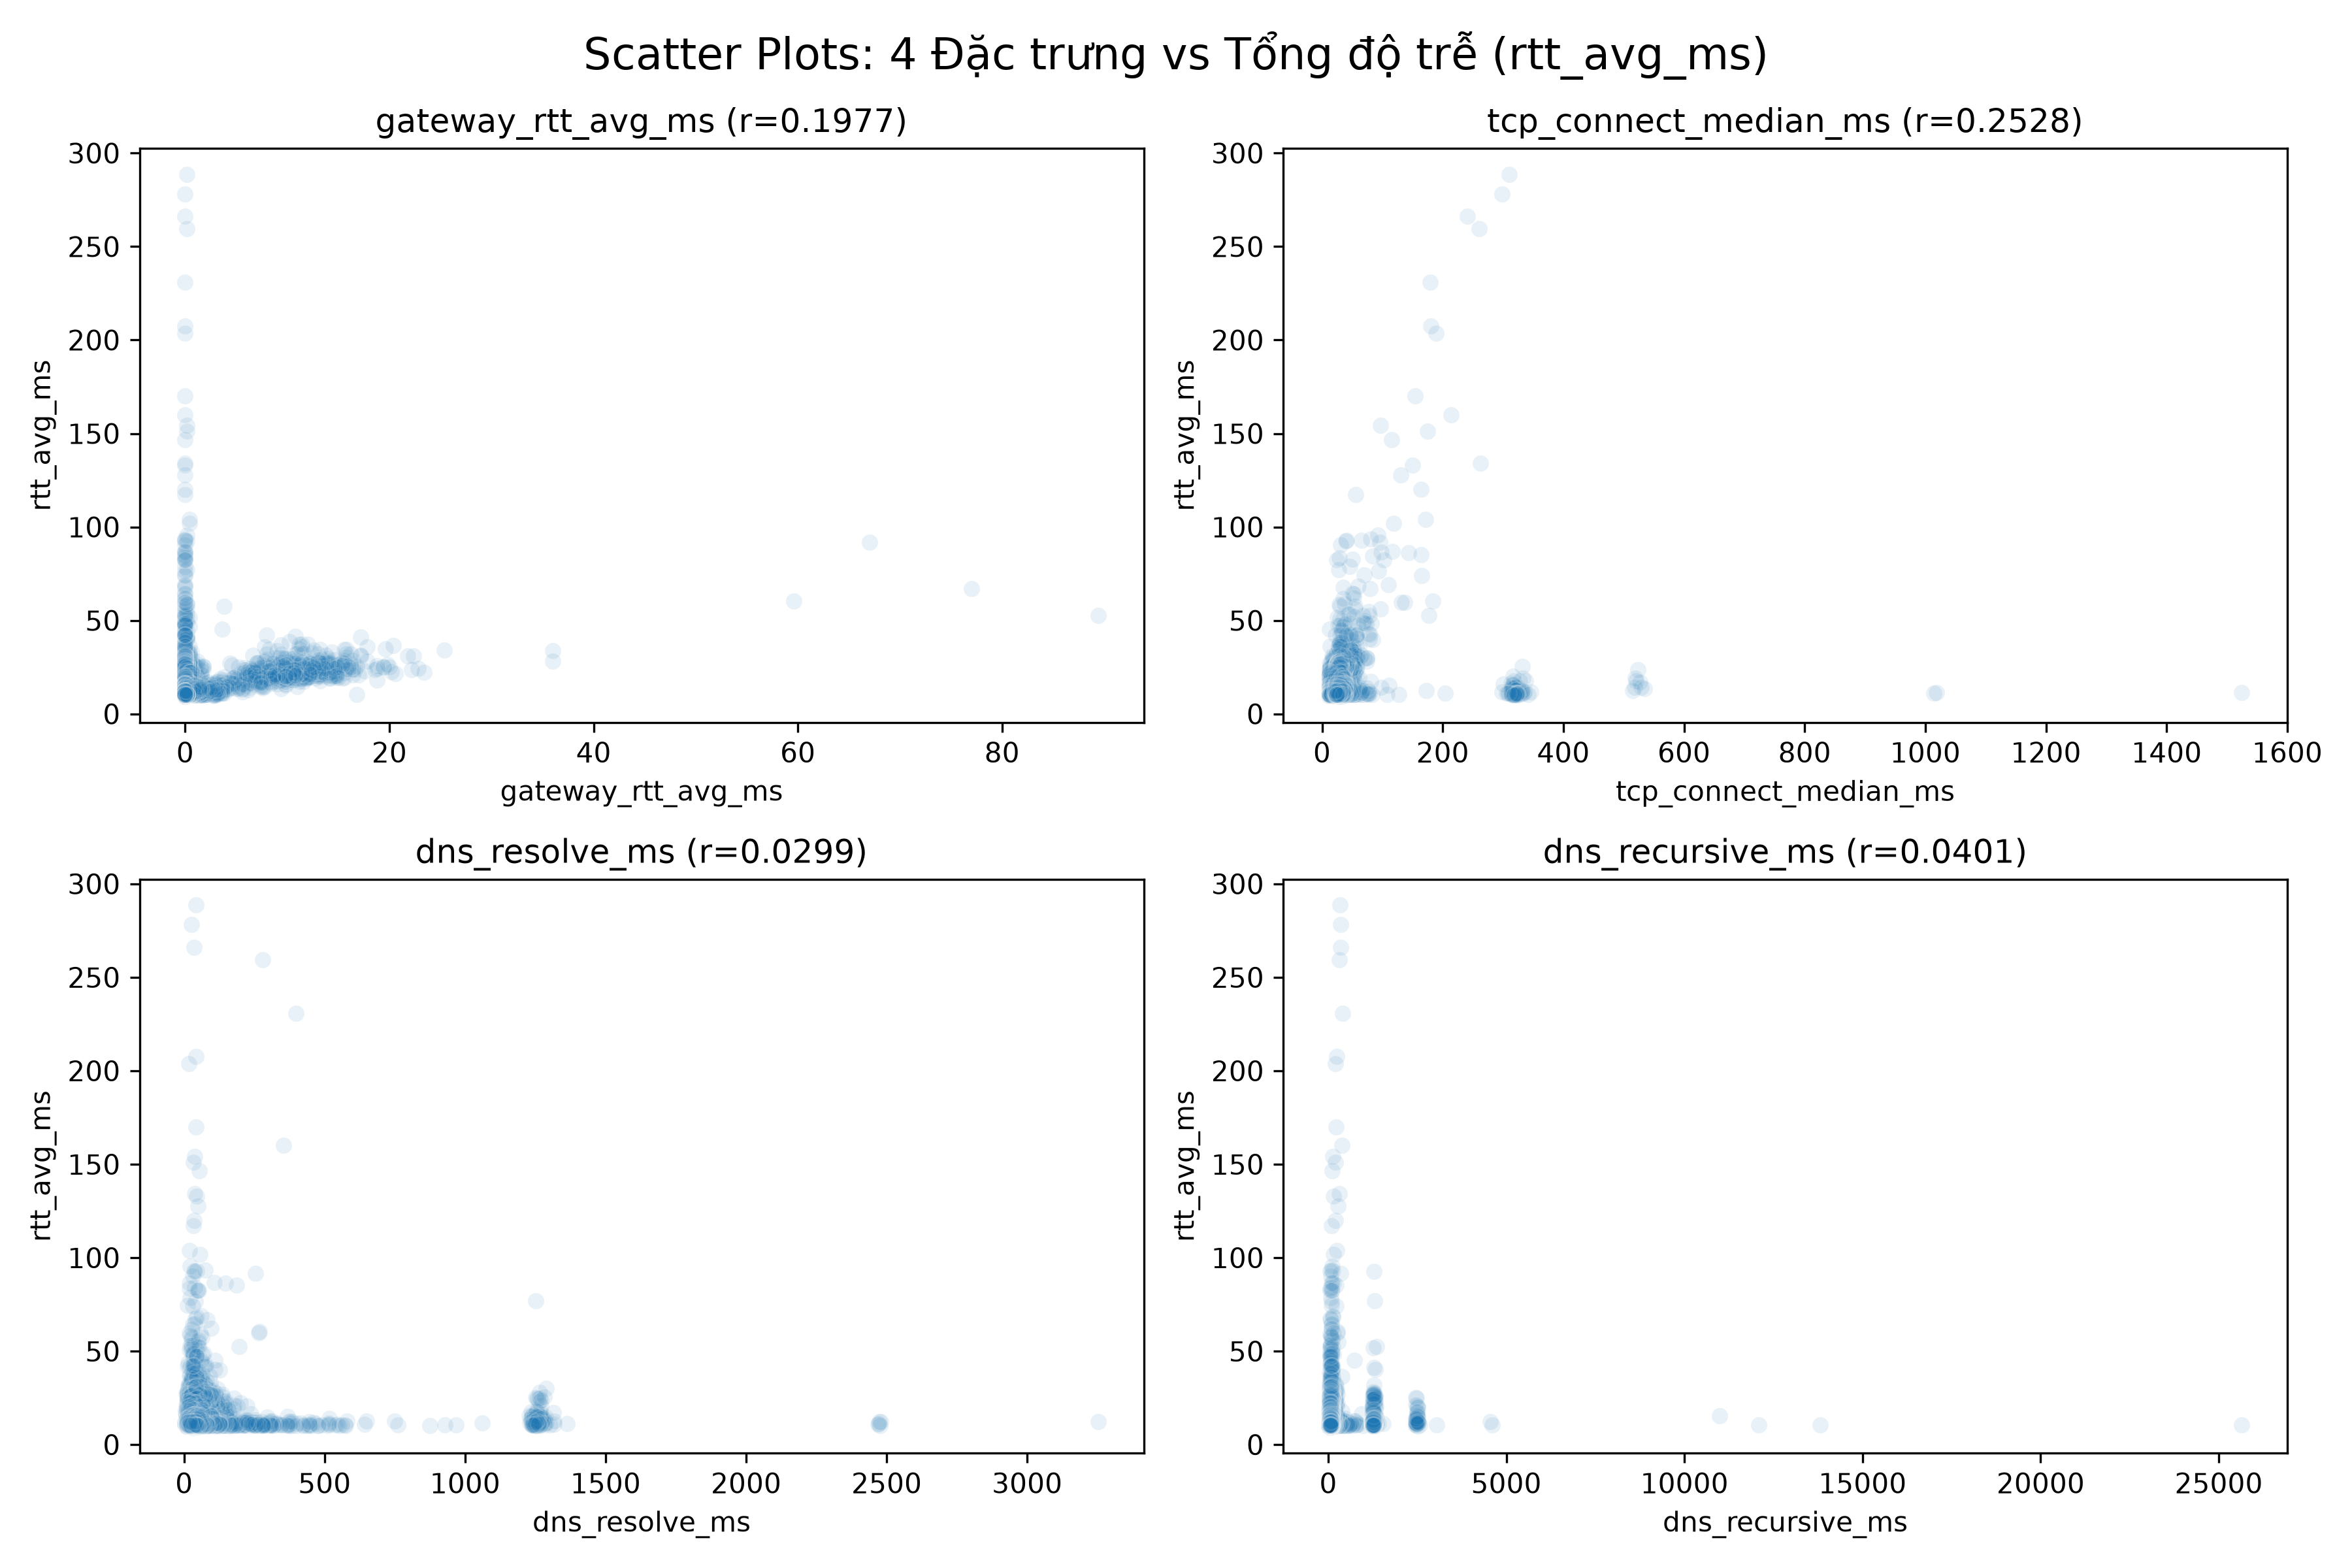
\includegraphics[width=1\textwidth]{Task2_Compare_4_Features_ScatterPlots.png}
    \caption{Biểu đồ phân tán so sánh 4 đặc trưng đầu vào với biến mục tiêu (\texttt{rtt\_avg\_ms})}
    \label{fig:scatter_4features}
\end{figure}

Từ Hình \ref{fig:scatter_4features}, ta có thể phân tích chi tiết bản chất của từng đặc trưng:
\begin{itemize}
    \item \textbf{Đặc trưng \texttt{gateway\_rtt\_avg\_ms} (Góc trên, trái):} Đồ thị thể hiện một hình chữ "L" đặc trưng. Điểm đáng chú ý nhất là có tới $25.221$ mẫu quan sát (chiếm gần một nửa tập dữ liệu) có giá trị \texttt{gateway\_rtt\_avg\_ms} bằng $0$ (Zeros = 25221). Điều này phản ánh thực tế mạng: tín hiệu gửi đến gateway (bộ định tuyến trong nhà) gần như diễn ra ngay tức khắc ($< 1$ ms). Tuy nhiên, tại chính mốc hoành độ $x=0$ này, trục tung $y$ lại phân tán dữ dội từ $10$ ms vọt thẳng lên $300$ ms. Đây chính là minh chứng trực quan cho thấy: mạng ở nhà (gateway) có thể hoàn toàn bình thường, nhưng gói tin vẫn bị trễ nghiêm trọng do nghẽn mạng quốc tế. Dạng phân bố này chắc chắn sẽ gây ra sai số lớn cho đường thẳng hồi quy tuyến tính.
    
    \item \textbf{Đặc trưng \texttt{tcp\_connect\_median\_ms} (Góc trên, phải):} Đây là biến có xu hướng tuyến tính rõ rệt nhất ($r \approx 0.2459$). Số lượng điểm Zeros bằng $0$, nghĩa là mọi kết nối TCP đều mất một khoảng thời gian nhất định để thiết lập (handshake). Các điểm dữ liệu bám theo một đường chéo dốc lên khá đồng đều, cho thấy thời gian thiết lập TCP tỷ lệ thuận khá tốt với tổng độ trễ.
    
    \item \textbf{Đặc trưng \texttt{dns\_resolve\_ms} và \texttt{dns\_recursive\_ms} (Hàng dưới):} Hai biểu đồ này thể hiện sự phân tán ngẫu nhiên, không có hình khối cụ thể. Hệ số tương quan cực kỳ thấp ($r < 0.05$) khẳng định thời gian phân giải tên miền (DNS) diễn ra độc lập và hiếm khi là nguyên nhân chính ảnh hưởng đến tổng độ trễ truyền tải của cả gói tin.
\end{itemize}
 % Hàm chi phí (Cost Function)
\section{Hàm chi phí (Cost Function)}

Để đánh giá mức độ sai lệch giữa mô hình dự đoán và dữ liệu thực tế, nhóm sử dụng hàm mất mát toàn phương trung bình (MSE Cost Function). Đối với mô hình hồi quy tuyến tính đơn biến, phương trình hàm giả thuyết được biểu diễn dưới dạng ma trận:
\begin{equation}
    f_\theta(\mathbf{x}) = \theta_0 + \theta_1 x_1 = X\theta
\end{equation}

Hàm chi phí $J(\theta)$ đo lường sai số bình phương trung bình trên tập dữ liệu gồm $n$ quan sát:
\begin{equation}
    J(\theta) = \frac{1}{2n}\sum_{i=1}^{n}\left(f_{\theta}(\mathbf{x}^{(i)}) - y^{(i)}\right)^2 = \frac{1}{2n}\|X\theta - y\|_2^2
\end{equation}

\textbf{Thực nghiệm trên tập huấn luyện (Train set):} Sau khi phân chia dữ liệu, tập huấn luyện có kích thước $n = 43.679$ mẫu. Ma trận thiết kế $X$ có kích thước $(43679 \times 2)$ (đã bổ sung cột bias). Khi khởi tạo tham số ban đầu $\theta_0 = 0$ và $\theta_1 = 0$, mức độ sai lệch ban đầu được hệ thống tính toán là $J(\theta) \approx 92.167$. Mục tiêu của quá trình tối ưu là tìm ra bộ tham số $\theta$ để giảm thiểu giá trị $J(\theta)$ này xuống mức thấp nhất có thể.


\section{Cài đặt Gradient Descent}

Gradient Descent (GD) là thuật toán tối ưu hóa lặp, được sử dụng để tìm kiếm điểm cực tiểu địa phương của một hàm khả vi.

\subsection{Quy tắc cập nhật và Đạo hàm}
Quy tắc cập nhật tham số $\theta$ di chuyển ngược hướng với gradient của hàm chi phí, được kiểm soát bởi tốc độ học (learning rate) $\gamma > 0$:
\begin{equation}
    \theta := \theta - \gamma \nabla_{\theta}J(\theta)^\top
\end{equation}

Trong đó, vector đạo hàm riêng (gradient) được biểu diễn dưới dạng ma trận tối ưu như sau:
\begin{equation}
    \nabla_{\theta}J(\theta)^\top = \frac{1}{n}X^\top(X\theta - y)
\end{equation}

\subsection{Quá trình hội tụ thực nghiệm}
Nhóm tiến hành cài đặt thuật toán GD trên tập huấn luyện với cấu hình: tốc độ học $\gamma = 0.01$ và giới hạn $1000$ vòng lặp (iterations). Kết quả theo dõi sự thay đổi của hàm chi phí và tham số qua các vòng lặp trọng điểm được ghi nhận như sau:

\begin{itemize}
    \item \textbf{Giai đoạn đầu (Vòng 1 - 100):} Hàm chi phí $J(\theta)$ giảm rất nhanh từ $92.16$ xuống mức $22.49$. Tham số $\theta_0$ tăng nhanh chóng lên mức $7.68$. Tốc độ giảm sâu này là đặc trưng của GD khi điểm hiện tại đang nằm xa đáy cực tiểu, độ dốc (gradient) lớn nên bước nhảy dài.
    \item \textbf{Giai đoạn giữa (Vòng 100 - 500):} Tốc độ giảm bắt đầu chậm lại khi hàm chi phí chạm mức $12.43$. Tham số $\theta_0$ vượt ngưỡng $12.18$.
    \item \textbf{Giai đoạn cuối (Vòng 500 - 1000):} Thuật toán gần như hội tụ hoàn toàn. Sự thay đổi của hàm chi phí trong 500 vòng lặp cuối là cực kỳ nhỏ (chỉ giảm từ $12.431$ xuống $12.424$). Tham số tối ưu cuối cùng chốt lại ở mức: $\theta_0 \approx 12.313$ và $\theta_1 \approx 0.831$.
\end{itemize}

Việc hàm chi phí tiến sát đến một giá trị giới hạn cố định chứng minh thuật toán đã thành công tìm được nghiệm cực tiểu toàn cục của không gian hồi quy.
 % Cài đặt Gradient Descent
\section{Nghiệm bình phương tối thiểu (Analytical Least-Squares Solution)}

Bên cạnh phương pháp lặp Gradient Descent (GD) dựa trên đạo hàm, bài toán hồi quy tuyến tính còn có thể được giải quyết triệt để bằng phương pháp đại số tuyến tính để tìm ra nghiệm chính xác tuyệt đối (closed-form solution). 

\subsection{Cơ sở toán học: Phương trình chuẩn (Normal Equations)}
Mục tiêu của tối ưu hóa là tìm điểm cực tiểu của hàm chi phí $J(\theta)$. Theo nguyên lý vi tích phân, tại điểm cực tiểu, đạo hàm của hàm chi phí theo vector tham số $\theta$ phải bằng 0. 

Cho đạo hàm $\nabla_{\theta}J(\theta) = 0$, ta thu được hệ Phương trình chuẩn (Normal Equations):
\begin{equation}
    (X^\top X)\theta = X^\top y \implies \theta^* = (X^\top X)^{-1} X^\top y
\end{equation}

\textit{Trong đó:}
\begin{itemize}
    \item $X$: Ma trận thiết kế chứa các đặc trưng đầu vào (kích thước $m \times (n+1)$).
    \item $y$: Vector cột chứa các giá trị thực tế của biến mục tiêu.
    \item $\theta^*$: Vector tham số tối ưu toán học.
    \item $(X^\top X)^{-1}$: Ma trận nghịch đảo của tích $X^\top X$.
\end{itemize}
Việc tính toán $\theta^*$ thông qua phương trình này mang lại nghiệm chính xác ngay trong một bước tính toán duy nhất, không cần chọn learning rate ($\gamma$) hay lặp nhiều vòng như thuật toán GD. Nhóm đã sử dụng hàm \texttt{np.linalg.inv} của thư viện NumPy để lập trình phép tính ma trận nghịch đảo này.

\subsection{Kết quả thực nghiệm và So sánh tham số}
Để kiểm chứng tính chính xác của thuật toán Gradient Descent tự cài đặt ở phần trước, nhóm tiến hành tính toán nghiệm giải tích trên cùng tập huấn luyện (Train set) và xuất ra kết quả so sánh. Từ Console Output, ta có những phân tích chuyên sâu sau:

\begin{itemize}
    \item \textbf{Về bộ tham số tối ưu ($\theta$):}
    \begin{itemize}
        \item Nghiệm từ Gradient Descent (sau 1000 vòng lặp): $\theta_0 \approx 12.3131, \theta_1 \approx 0.8314$
        \item Nghiệm Giải tích (Nghiệm đúng): $\theta_0 \approx 12.3146, \theta_1 \approx 0.8309$
    \end{itemize}
    \textbf{Giải thích ý nghĩa:} Hai bộ tham số này gần như trùng khớp hoàn toàn, chỉ chênh lệch ở chữ số thập phân thứ 3. Sự chênh lệch siêu nhỏ này xuất phát từ bản chất của phương pháp: Gradient Descent là thuật toán \textit{tối ưu lặp (tiệm cận)}. Thuật toán dừng lại ở vòng lặp 1000 khi tham số đã "bò" xuống rất sát đáy lòng chảo; trong khi đó, Phương trình chuẩn sử dụng ma trận nghịch đảo để nhảy thẳng tới tâm đáy \textit{chính xác tuyệt đối về mặt toán học}.
    
    \item \textbf{Về sai lệch hàm chi phí (Cost Difference = 1.11e-06):}
    Hệ thống ghi nhận sự chênh lệch giá trị Cost ($J(\theta)$) giữa hai phương pháp là \texttt{1.11e-06} (tức là $0.00000111$). Con số này thực chất là độ lệch giữa mức sai số của GD (khi dừng ở vòng 1000) so với mức sai số lý tưởng toán học.
    \\
    \textbf{Nguyên nhân và Kết luận:} Mức chênh lệch $1.11 \times 10^{-6}$ này là một giá trị cực kỳ nhỏ (gần bằng $0$). Điều này minh chứng hùng hồn cho hai yếu tố quan trọng:
    \begin{enumerate}
        \item Thuật toán Gradient Descent mà nhóm tự lập trình từ đầu (scratch) hoạt động hoàn toàn chính xác.
        \item Các siêu tham số (Hyperparameters) được cấu hình trong GD bao gồm learning rate $\gamma = 0.01$ và $1000$ vòng lặp là cực kỳ hợp lý, vừa đủ để thuật toán hội tụ mượt mà về đúng điểm cực tiểu toàn cục của hàm mất mát, không bị văng (phân kỳ) cũng không bị dừng quá sớm.
    \end{enumerate}
\end{itemize}
 % Nghiệm bình phương tối thiểu & Bề mặt hàm chi phí
% =========================================================
% BÀI 6: PHÂN TÍCH HỘI TỤ (CONVERGENCE ANALYSIS)
% =========================================================
\section{Phân tích hội tụ (Convergence Analysis)}

\subsection{Mục tiêu}
Đánh giá tốc độ hội tụ của thuật toán Gradient Descent thông qua việc biểu diễn giá trị hàm chi phí \(J(\boldsymbol{\theta})\) theo số vòng lặp (iterations). Đồng thời, thực hiện so sánh thực nghiệm để lựa chọn ra tốc độ học (Learning Rate - LR) tối ưu nhất.

\subsection{Kết quả thực hiện}

\chenhinh{figures/7_convergence.png}
{Giá trị hàm chi phí theo số vòng lặp với các mức Learning Rate khác nhau}
{fig:convergence}

\subsection{Phân tích chi tiết}
Để tìm ra Learning Rate phù hợp nhất, nhóm đã tiến hành chạy thực nghiệm thuật toán với 3 mức LR khác nhau: \(0.001\), \(0.01\) và \(0.1\) trên cùng \(3000\) vòng lặp. Kết quả được thể hiện qua 3 đường trên biểu đồ:

\begin{itemize}
    \item \textbf{LR = 0.001 (Đường màu đỏ - Quá chậm):} Đường cong Cost giảm từ từ với độ dốc thấp. Sau \(3000\) vòng lặp, giá trị Cost vẫn chưa chạm tới mức tối ưu (đường nét đứt đen). Điều này cho thấy LR quá nhỏ khiến mô hình học quá chậm và lãng phí tài nguyên tính toán.
    
    \item \textbf{LR = 0.1 (Đường màu xanh lá - Quá nhanh):} Mô hình lao dốc cực nhanh và chạm đáy chỉ sau khoảng \(100\) vòng lặp đầu tiên. Tuy nhiên, bước nhảy quá lớn (large step size) tiềm ẩn rủi ro dao động mạnh (zig-zag) hoặc phân kỳ (văng ra ngoài không gian nghiệm) nếu dữ liệu đầu vào không được chuẩn hóa tốt.
    
    \item \textbf{LR = 0.01 (Đường màu xanh dương - Tối ưu):} Đây là mức Learning Rate được nhóm lựa chọn. Đường cong Cost giảm rất nhanh nhưng vẫn giữ được độ mượt mà, không bị dao động. Kết quả phân tích bằng thuật toán quét cho thấy, mô hình đạt mức tối ưu (sai số \(< 0.001\) so với Normal Equation) ngay tại vòng lặp thứ \(617\).
\end{itemize}

\subsection{Kết luận}
Việc lựa chọn Learning Rate ảnh hưởng trực tiếp đến hiệu suất của mô hình. Với dữ liệu đã được chuẩn hóa (StandardScaler), LR = 0.01 là sự cân bằng hoàn hảo nhất giữa tốc độ hội tụ và tính ổn định. Thuật toán Gradient Descent đã hội tụ hoàn toàn với sai lệch Cost so với nghiệm giải tích chỉ còn \(0.00 \times 10^0\) (gần như bằng 0 tuyệt đối). % Phân tích hội tụ (Convergence Analysis)
% =========================================================
% BÀI 7: PHÂN TÍCH HỘI TỤ (CONVERGENCE ANALYSIS)
% =========================================================
\section{Convergence analysis}

\subsection{Mục tiêu}
Đánh giá tốc độ hội tụ của thuật toán Gradient Descent thông qua việc biểu diễn giá trị hàm chi phí \(J(\boldsymbol{\theta})\) theo số vòng lặp (iterations). Đồng thời, thực hiện so sánh thực nghiệm để lựa chọn ra tốc độ học (Learning Rate - LR) tối ưu nhất.

\subsection{Kết quả thực hiện}

% Nhớ lưu ảnh biểu đồ đường (Learning Rate) vào thư mục figures/ với đúng tên dưới đây
\chenhinh{figures/07.jpg}
{Giá trị hàm chi phí theo số vòng lặp với các mức Learning Rate khác nhau}
{fig:convergence}

\subsection{Phân tích chi tiết}
Để tìm ra Learning Rate phù hợp nhất, nhóm đã tiến hành chạy thực nghiệm thuật toán với 3 mức LR khác nhau: \(0.001\), \(0.01\) và \(0.1\) trên cùng \(3000\) vòng lặp. Kết quả được thể hiện qua 3 đường trên biểu đồ:

\begin{itemize}
    \item \textbf{LR = 0.001 (Đường màu đỏ - Quá chậm):} Đường cong Cost giảm từ từ với độ dốc thấp. Sau \(3000\) vòng lặp, giá trị Cost vẫn chưa chạm tới mức tối ưu (đường nét đứt đen). Điều này cho thấy LR quá nhỏ khiến mô hình học quá chậm và lãng phí tài nguyên tính toán.
    
    \item \textbf{LR = 0.1 (Đường màu xanh lá - Quá nhanh):} Mô hình lao dốc cực nhanh và chạm đáy chỉ sau khoảng \(100\) vòng lặp đầu tiên. Tuy nhiên, bước nhảy quá lớn (large step size) tiềm ẩn rủi ro dao động mạnh (zig-zag) hoặc phân kỳ (văng ra ngoài không gian nghiệm) nếu dữ liệu đầu vào không được chuẩn hóa tốt.
    
    \item \textbf{LR = 0.01 (Đường màu xanh dương - Tối ưu):} Đây là mức Learning Rate được nhóm lựa chọn. Đường cong Cost giảm rất nhanh nhưng vẫn giữ được độ mượt mà, không bị dao động. Kết quả phân tích bằng thuật toán quét cho thấy, mô hình đạt mức tối ưu (sai số \(< 0.001\) so với Normal Equation) ngay tại vòng lặp thứ \(617\).
\end{itemize}

\subsection{Kết luận}
Việc lựa chọn Learning Rate ảnh hưởng trực tiếp đến hiệu suất của mô hình. Với dữ liệu đã được chuẩn hóa (StandardScaler), LR = 0.01 là sự cân bằng hoàn hảo nhất giữa tốc độ hội tụ và tính ổn định. Thuật toán Gradient Descent đã hội tụ hoàn toàn với sai lệch Cost so với nghiệm giải tích chỉ còn \(0.00 \times 10^0\) (gần như bằng 0 tuyệt đối). % Dự đoán, đánh giá mô hình và phân tích phần dư
\subsection{Đánh giá mô hình và so sánh tham số (Console Output)}
Kết quả huấn luyện và đánh giá trên tập kiểm tra (Test set) cho thấy sự tương đồng gần như tuyệt đối giữa thuật toán Gradient Descent (GD) tự cài đặt và nghiệm giải tích (Analytical Solution).
\begin{itemize}
    \item \textbf{Sự hội tụ của tham số:} Tham số thu được từ NumPy GD ($\theta_0 \approx 12.313, \theta_1 \approx 0.831$) khớp đến chữ số thập phân thứ ba so với nghiệm giải tích ($\theta_0 \approx 12.314, \theta_1 \approx 0.830$). Điều này chứng minh thuật toán Gradient Descent đã được lập trình chính xác và hội tụ thành công về điểm cực tiểu toàn cục.
    \item \textbf{Đánh giá sai số:} Sai số toàn phương trung bình (MSE) của cả hai phương pháp đều đạt mức xấp xỉ $31.35$.
    \item \textbf{Hệ số xác định ($R^2$):} Mức $R^2 \approx 0.021$ (tức 2.1\%) không phải là lỗi của mô hình, mà phản ánh đúng bản chất của tập dữ liệu thực tế. Biến đầu vào \texttt{gateway\_rtt\_avg\_ms} chỉ giải thích được 2.1\% sự biến thiên của \texttt{rtt\_avg\_ms}. Về mặt vật lý mạng, độ trễ đến gateway nội bộ thường rất nhỏ và ổn định, trong khi tổng độ trễ đến máy chủ đích phụ thuộc chủ yếu vào trạng thái đường truyền Internet bên ngoài. Do đó, việc chỉ dùng gateway RTT để dự đoán tổng RTT sinh ra độ chính xác thấp.
\end{itemize}

\subsection{Trực quan hóa đường hồi quy và phân tích phần dư}
\begin{itemize}
    \item \textbf{Biểu đồ so sánh hồi quy (Regression Comparison):} Hầu hết các điểm dữ liệu thực tế (chấm xanh dương) tập trung cực kỳ dày đặc ở khu vực $x \approx 0$, nhưng giá trị độ trễ thực tế ($y$) tại đó lại phân tán mạnh, có những điểm vọt lên gần $300$ ms. Đường hồi quy tuyến tính bị kéo lệch bởi cụm điểm dày đặc ở trọng tâm (mức $\approx 12$ ms) và nỗ lực bám theo các điểm ngoại lai lác đác ở phía xa ($x \approx 90$), tạo ra độ dốc tương đối thoải $\theta_1 \approx 0.83$.
    
    \item \textbf{Hai biểu đồ phần dư (NumPy GD Residuals \& Analytical Residuals):} Hai biểu đồ này có sự phân bố điểm ảnh giống hệt nhau, một lần nữa khẳng định thuật toán GD tự cài đặt đã tìm ra tham số chính xác như công thức toán học.
    \begin{itemize}
        \item \textit{Trục hoành (Predicted RTT):} Thể hiện giá trị dự đoán của mô hình ($\hat{y}$). Vì đặc thù dữ liệu đầu vào $x$ (trễ gateway) phần lớn xoay quanh mức $0$ ms, phương trình hồi quy chủ yếu trả về kết quả dự đoán bằng đúng hệ số chặn ($\hat{y} \approx 12.31$ ms). Điều này tạo ra một cột dữ liệu tập trung dày đặc theo chiều dọc ngay tại hoành độ $12$ ms.
        \item \textit{Trục tung (Residual):} Thể hiện mức độ sai số ($e = y - \hat{y}$). Đường đứt nét màu đỏ ngang mốc $0$ là mức lý tưởng (dự đoán khớp hoàn toàn với thực tế). Tuy nhiên, tại cột mốc dự đoán $12$ ms, phần dư không phân bố đều quanh số $0$ mà kéo vọt lên thành một vệt thẳng đứng tới gần $300$ ms.
        \item \textit{Ý nghĩa phân tích:} Sự phân bố dị biệt này chứng tỏ phương sai sai số không đồng đều (heteroscedasticity). Về mặt thực tế, khi gateway phản hồi cực nhanh ($0$ ms), mô hình tự tin đoán tổng độ trễ là $12$ ms. Tuy nhiên, gói tin thỉnh thoảng vẫn bị "lag" đột biến lên $300$ ms do nghẽn mạng quốc tế hoặc máy chủ đích. Mô hình không có dữ liệu để lường trước cú lag này, dẫn đến sai số khổng lồ $e \approx 300 - 12 = 288$ ms.
        \item Ngược lại, một vài điểm ngoại lai nằm rải rác bên phải ($\hat{y} > 40$ ms) lại có phần dư khá nhỏ (bám sát đường màu đỏ). Điều này cho thấy: mô hình chỉ đoán trúng khi bản thân mạng cục bộ (gateway) thực sự bị chậm, nhưng lại hoàn toàn "mù" trước các nguyên nhân gây trễ từ môi trường Internet bên ngoài.
    \end{itemize}
\end{itemize}

\subsection{Giải thích hiện tượng trùng khớp đường đồ thị}
Trên góc phải của biểu đồ Regression Comparison, chú giải (legend) ghi nhận sự tồn tại của hai đường biểu diễn: NumPy GD (màu đỏ) và Analytical (màu xanh lá). Tuy nhiên, trên đồ thị thực tế chỉ quan sát thấy duy nhất đường màu xanh lá. 

Nguyên nhân xuất phát từ việc bộ tham số $\theta$ của hai phương pháp gần như giống hệt nhau, khiến hai đường thẳng có cùng hệ số góc và tung độ gốc, nằm trùng khít lên nhau. Trong mã nguồn trực quan hóa, lệnh vẽ đường Analytical (\texttt{color="green"}) được thực thi ngay sau lệnh vẽ đường NumPy GD (\texttt{color="red"}). Do đó, thư viện Matplotlib đã render lớp màu xanh lá đè lên trên, che khuất hoàn toàn đường hồi quy màu đỏ ở bên dưới.

\subsection{Cơ sở toán học và phương pháp tính toán thông số}
Toàn bộ các chỉ số đánh giá và dữ liệu vẽ đồ thị được lập trình dựa trên các công thức đại số tuyến tính và thống kê cốt lõi sau:
\begin{itemize}
    \item \textbf{Giá trị dự đoán ($\hat{y}$):} Được tính bằng phép nhân ma trận giữa ma trận thiết kế $X$ (đã bổ sung vector cột chứa toàn số $1$) và vector tham số $\theta$:
    \begin{equation}
        \hat{y} = X\theta = \theta_0 + \theta_1 x_1
    \end{equation}
    \textit{Trong đó:}
    \begin{itemize}
        \item $\hat{y}$: Tổng độ trễ dự đoán tới máy chủ đích (\texttt{rtt\_avg\_ms}), đơn vị là mili-giây (ms).
        \item $X$: Ma trận thiết kế đầu vào (chứa các giá trị $x_1$ và cột số $1$).
        \item $\theta_0$: Hệ số chặn (Intercept), là giá trị trễ dự đoán khi $x_1 = 0$, đơn vị là ms.
        \item $\theta_1$: Hệ số góc (Slope), thể hiện sự thay đổi của $\hat{y}$ khi $x_1$ tăng thêm 1 đơn vị.
        \item $x_1$: Đặc trưng đầu vào độ trễ gateway (\texttt{gateway\_rtt\_avg\_ms}), đơn vị là ms.
    \end{itemize}

    \item \textbf{Sai số toàn phương trung bình (MSE - Mean Squared Error):} Đo lường trung bình cộng của bình phương các khoảng cách từ điểm dữ liệu thực tế đến đường hồi quy dự đoán:
    \begin{equation}
        \text{MSE} = \frac{1}{m} \sum_{i=1}^{m} \left(y^{(i)} - \hat{y}^{(i)}\right)^2
    \end{equation}
    \textit{Trong đó:}
    \begin{itemize}
        \item $m$: Tổng số lượng mẫu (quan sát) có trong tập dữ liệu kiểm tra (Test set).
        \item $y^{(i)}$: Giá trị độ trễ thực tế của quan sát thứ $i$, đơn vị là ms.
        \item $\hat{y}^{(i)}$: Giá trị độ trễ do mô hình dự đoán tại quan sát thứ $i$, đơn vị là ms.
        \item $\sum_{i=1}^{m}$: Ký hiệu tổng cộng dồn từ quan sát đầu tiên ($i=1$) đến quan sát cuối cùng ($i=m$).
    \end{itemize}

    \item \textbf{Hệ số xác định ($R^2$ Score):} Đánh giá tỷ lệ phương sai của biến mục tiêu được giải thích bởi mô hình. Chỉ số này so sánh sai số của mô hình hiện tại với sai số giả định nếu chỉ dùng giá trị trung bình $\bar{y}$ để dự đoán:
    \begin{equation}
        R^2 = 1 - \frac{\sum_{i=1}^{m} \left(y^{(i)} - \hat{y}^{(i)}\right)^2}{\sum_{i=1}^{m} \left(y^{(i)} - \bar{y}\right)^2}
    \end{equation}
    \textit{Trong đó:}
    \begin{itemize}
        \item Tử số $\sum (y^{(i)} - \hat{y}^{(i)})^2$: Tổng bình phương phần dư (RSS), thể hiện mức độ sai số của mô hình.
        \item Mẫu số $\sum (y^{(i)} - \bar{y})^2$: Tổng bình phương toàn phần (TSS), thể hiện mức độ phân tán của dữ liệu gốc.
        \item $\bar{y}$: Giá trị độ trễ trung bình của toàn bộ các điểm thực tế trong tập kiểm tra, đơn vị là ms.
    \end{itemize}

    \item \textbf{Phần dư (Residuals):} Là sự chênh lệch trực tiếp giữa giá trị thực tế và giá trị dự đoán, được sử dụng làm tung độ cho hai biểu đồ phân tích phần dư:
    \begin{equation}
        e^{(i)} = y^{(i)} - \hat{y}^{(i)}
    \end{equation}
    \textit{Trong đó:}
    \begin{itemize}
        \item $e^{(i)}$: Mức độ sai lệch (phần dư) của riêng quan sát thứ $i$. Đơn vị là ms. Nếu $e^{(i)} > 0$, mô hình đang dự đoán thấp hơn thực tế; ngược lại nếu $e^{(i)} < 0$, mô hình đang dự đoán cao hơn thực tế.
    \end{itemize}
\end{itemize}
 % So sánh với thư viện (Scikit-learn)
\input{chapters/bai_09} % Cải thiện mô hình (Model Improvement)
\input{chapters/bai_10} % Kết luận (Conclusion)

% =========================================================
% 5. TÀI LIỆU THAM KHẢO
% =========================================================
\clearpage
\phantomsection
\addcontentsline{toc}{section}{Tài liệu tham khảo}
\printbibliography

% =========================================================
% 6. PHỤ LỤC (Nếu muốn tách riêng có thể tạo chapters/phu_luc.tex)
% =========================================================
\clearpage
\appendix
\input{chapters/phu_luc} % Chứa mã nguồn và phân công công việc

\end{document}